% Rappresenta il tipo di documento
\documentclass[12pt, twoside]{book}

% Elenco dei packages utilizzati
\usepackage[a4paper,width=150mm,top=25mm,bottom=25mm,bindingoffset=6mm]{geometry}
\usepackage[utf8]{inputenc}
\usepackage[T1]{fontenc}
\usepackage[italian]{babel}
\usepackage{subcaption}
\usepackage{graphicx}
\usepackage{fancyhdr}
\usepackage{float}
\usepackage{color}
\usepackage[nottoc]{tocbibind}
\usepackage{emptypage}
\usepackage[hidelinks]{hyperref}
\usepackage{titlesec}
\usepackage{amssymb}
\usepackage[sorting=none,backend=bibtex]{biblatex}
\usepackage{csquotes}
\usepackage{pdfpages}
\usepackage{amsmath}
\usepackage{placeins}
\usepackage{hyperref}
\usepackage{footnote}
% Stile di pagina
\setlength{\parindent}{0em}
\setlength{\parskip}{0.5em}

\renewcommand{\chaptermark}[1]{\markboth{#1}{}}
\renewcommand{\tocetcmark}[1]{\markboth{#1}{}}
\renewcommand{\sectionmark}[1]{\markright{\thesection\ #1}}
\fancyhf{}
\fancyhead[LE,RO]{\bfseries\thepage}
\fancyhead[LO]{\bfseries\rightmark}
\fancyhead[RE]{\bfseries\leftmark}
\renewcommand{\headrulewidth}{0.5pt}
\fancypagestyle{plain}{
    \fancyhead{}
    \renewcommand{\headrulewidth}{0pt}
}
\setlength{\headheight}{28pt}

% Stile dei titoli dei capitoli
\definecolor{gray75}{gray}{0.75}
\newcommand{\hsp}{\hspace{20pt}}
\titleformat{\chapter}[hang]
{\Huge\bfseries}
{\thechapter\hsp\textcolor{gray75}{|}\hsp}
{0pt}
{\Huge\bfseries}

% Impostazioni bibliografia
\addbibresource{./bibliografia/bibliografia.bib}

% Ridefinizione enfasi
%\DeclareTextFontCommand{\emph}{\bfseries\em}

% Inizio del documento
\begin{document}

% Frontespizio

\includepdf{./frontespizio/frontespizio.pdf}
% Introduzione
\chapter*{Introduzione}
\chaptermark{Introduzione}
\addcontentsline{toc}{chapter}{Introduzione}

L’implementazione di strumenti atti a combattere gli attacchi di tipo denial of service, sono ormai da molto tempo materia di studio e di ricerca. Questi attacchi possono rappresentare una minaccia grave, soprattutto quando si verificano su servizi cruciali e sensibili. Per tale motivo, negli anni sono state sviluppate molte strategie diverse per impedire ai singoli o ai gruppi di computer (noti anche come "zombie armies") di attaccare servizi o reti. Attualmente una delle metodologie di protezione più comuni agli attacchi DoS è il Rate-limiting, che permette di imporre una frequenza massima accettabile per le richieste, al fine di evitare sovraccarichi e congestionamenti delle risorse. In particolare, nei sistemi su larga scala, la limitazione della frequenza rappresenta uno strumento essenziale per garantire la disponibilità e l'integrità delle risorse e dei servizi.\par

Un altro campo di interesse in cui si sono fatti molti progressi negli ultimi anni, grazie soprattutto all'avvento delle tecnologie Block-chain, è stato quello dell’anonimato in rete. Con il termine anonimato in rete ci si riferisce alla condizione in cui, sulla base di una conoscenza parziale o totale delle interazioni di un utente su una rete, non è possibile risalire all'identità dell'utente stesso, permettendo un'interazione con i servizi offerti dalla rete in assoluta riservatezza. L'anonimato in rete presenta molteplici vantaggi, soprattutto in contesti in cui la privacy costituisce un requisito fondamentale, come ad esempio nelle votazioni o nelle transazioni finanziarie. Inoltre, la possibilità di mantenere l'anonimato può rivelarsi altrettanto utile in ambiti più diffusi come le conversazioni online o sui social network, garantendo la libertà di espressione e la tutela della propria sfera privata.\par

Tuttavia, l'anonimato in rete presenta anche alcune criticità, tra cui la principale è rappresentata dalla difficoltà di controllo. La ragione è da individuare nel fatto che le metodologie di sicurezza a livello applicazione (pila ISO/OSI) generalmente si fondano sulla sorveglianza del comportamento degli utenti o dei dispositivi, nel corso del tempo, al fine di rilevare i pattern di attività che potrebbero suggerire la presenza di un attacco. In un contesto anonimo, in cui le identità degli utenti non sono tracciabili, ciò diviene notevolmente più arduo. Esistono strumenti di rate-limiting efficaci a livelli inferiori della pila ISO/OSI, come a livello di trasporto o di sessione. Tuttavia, la loro attuazione comporta alcuni svantaggi, come il rischio di limitare o bloccare numerosi indirizzi IP tradotti sotto una NAT, minare la privacy degli utenti disattivando le protezioni come TLS per effettuare DPI o ancora essere elusi da tecniche di mascheramento, come l'IP spoofing. Per tali motivazioni, per un servizio diffuso in ambiente anonimo, non è possibile fare affidamento esclusivamente su questi strumenti.\par
\clearpage
La presente tesi affronta la discussione di un protocollo chiamato RLN (Rate-Limiting Nullifier) basato sulla tecnologia zk-SNARK, che permette di attuare un rate-limiting in ambiente anonimo. Il protocollo si delinea in tre parti generali che si diversificano nei dettagli in base al dominio applicativo di utilizzo. \par

Fasi del protocollo:\par
\begin{itemize}
    \item \textbf{Registrazione:} Durante questa fase, gli utenti che desiderano accedere al servizio devono registrarsi fornendo una prova del possesso di determinati requisiti. Questa prova di possesso è denominata "identity commitment" e viene conservata e utilizzata nelle fasi successive del protocollo. I dati personali che soddisfano i requisiti sono definiti "stake" e possono assumere forme diverse a seconda del contesto applicativo. Ad esempio, possono essere costituiti da un profilo su un social network, dall'indirizzo di un portafoglio di criptovalute o da un'identità digitale come lo SPID o la CIE. 

    Gli stake non vengono conservati dal protocollo e, alla fine della fase di registrazione, l'informazione fornita al servizio consiste unicamente nel fatto che un nuovo utente anonimo che soddisfa le specifiche della registrazione è stato aggiunto al servizio.\par
    
    \item \textbf{Interazione:} Dopo essersi registrati, gli utenti hanno la possibilità di interagire con il servizio attraverso l'invio di richieste. Ad ogni richiesta, gli utenti sono tenuti a fornire una prova di appartenenza al sistema. Tale prova è generata tramite la tecnologia zk-SNARK, che consente di dimostrare al servizio che l'utente è effettivamente un membro legittimo senza rivelare alcuna informazione sulla sua identità. Inoltre, il protocollo consente di implementare una regola di rate-limiting, che, se non rispettata, porta l'utente a rivelare la propria stake. 
    
    Ciò consente di scoprire e gestire chi attua comportamenti di spam o Dos, e di procedere alla fase successiva.

    \item \textbf{Punizione:} La tipologia e il grado di punizione dipendono molto dal contesto applicativo. Ad esempio, alcune punizioni o misure di "slashing" possono comportare la rimozione del membro dal gruppo, con conseguente impossibilità di interagire con il sistema o la perdita dell'anonimato. In presenza di una stake, è possibile prevedere sanzioni più articolate, come l'inserimento dell'identità virtuale in un registro di esclusione per altri servizi, o la rivelazione dell'indirizzo del portafoglio criptovalute dell'utente e il sequestro dei fondi.
   
\end{itemize}
 Di seguito si cercherà di guardare a tutto tondo le tecnologie e le idee alla base di zk-Snark e del protocollo RLN. Inoltre si mostrerà l'implementazione di un piccolo prototipo che utilizza questo protocollo per evitare la sovraccarico delle risorse in un servizio basato su API.


% Capitoli
\chapter{Stato dell'arte}
\label{ch:state of the art}
\section{Denial-of-Service (DoS)}
\label{sec:Denial-of-Service (DoS)}
Gli attacchi di tipo Denial-of-Service (DoS) sono una tipologia di attacchi informatici estremamente diffusi, la cui
frequenza è cresciuta negli anni sia in termini quantitativi che qualitativi. Questo incremento è stato determinato
dalla relativa facilità con cui è possibile condurre un attacco di questo tipo, nonché dalle sue conseguenze, che in
base alle contromisure adottate e alla struttura del servizio attaccato possono essere più o meno gravi.
% \cite{google_ddos}
Nella tesi ci concentreremo solamente, sull'analisi della metodologia di protezione denominate rate-limiting. Queste
strategie possono risultare estremamente efficaci in alcune situazioni, come dimostrato dall'evento accaduto ad agosto
2022 a Google, che grazie all’attivazione di un rate-limiter è stato in grado di contrastare con
successo il più grande attacco di tipo DDoS a livello applicativo mai registrato. Tale attacco, proveniente da oltre
5.256 sorgenti IP dislocate in 132 paesi differenti, ha raggiunto il picco di 46 milioni di richieste al secondo.

In generale, un una regola per il rate limiting consiste in un semplice conteggio delle occorrenze delle richieste in un
lasso di tempo. Tuttavia, esistono diverse tecniche per misurare e limitare la frequenza di tali richieste, ognuna con i
propri usi e implicazioni.
\begin{itemize}
    \item \textbf{Fixed window :} L'obiettivo del training è combinare le rappresentazioni delle parole limitrofe per
     prevedere la parola centrale. Tra tutte le strategie che vedremo è la più semplice da implementare, consiste nello
     stabilire un limite massimo al numero di richieste che possono essere inviate in un determinato intervallo di
     tempo, detto "finestra". Ad esempio, si potrebbe limitare il numero di richieste a 100 ogni minuto. Questo limite
     viene applicato in modo uniforme all'interno della finestra temporale. Ciò significa che, una volta raggiunto il
     limite massimo di richieste consentite, l'utente o l'applicazione deve attendere il termine della finestra
     temporale per poter inviare nuove richieste. Uno svantaggio significativo di questa strategia è la possibile
     concentrazione di richieste tutte in una porzione della finestra, rischiando un sovraccarico del servizio. Caso
     notevole è quello in cui si concentrino tutte le richieste di una finestra al margine della fine e tutte le
     richieste della finestra successiva al margine dell’inizio questo comporta che il sistema in una durata equivalente
     a quella della finestra ha ricevuto il doppio delle richieste consentite.\clearpage
        \begin{figure}[H]
        \centering
        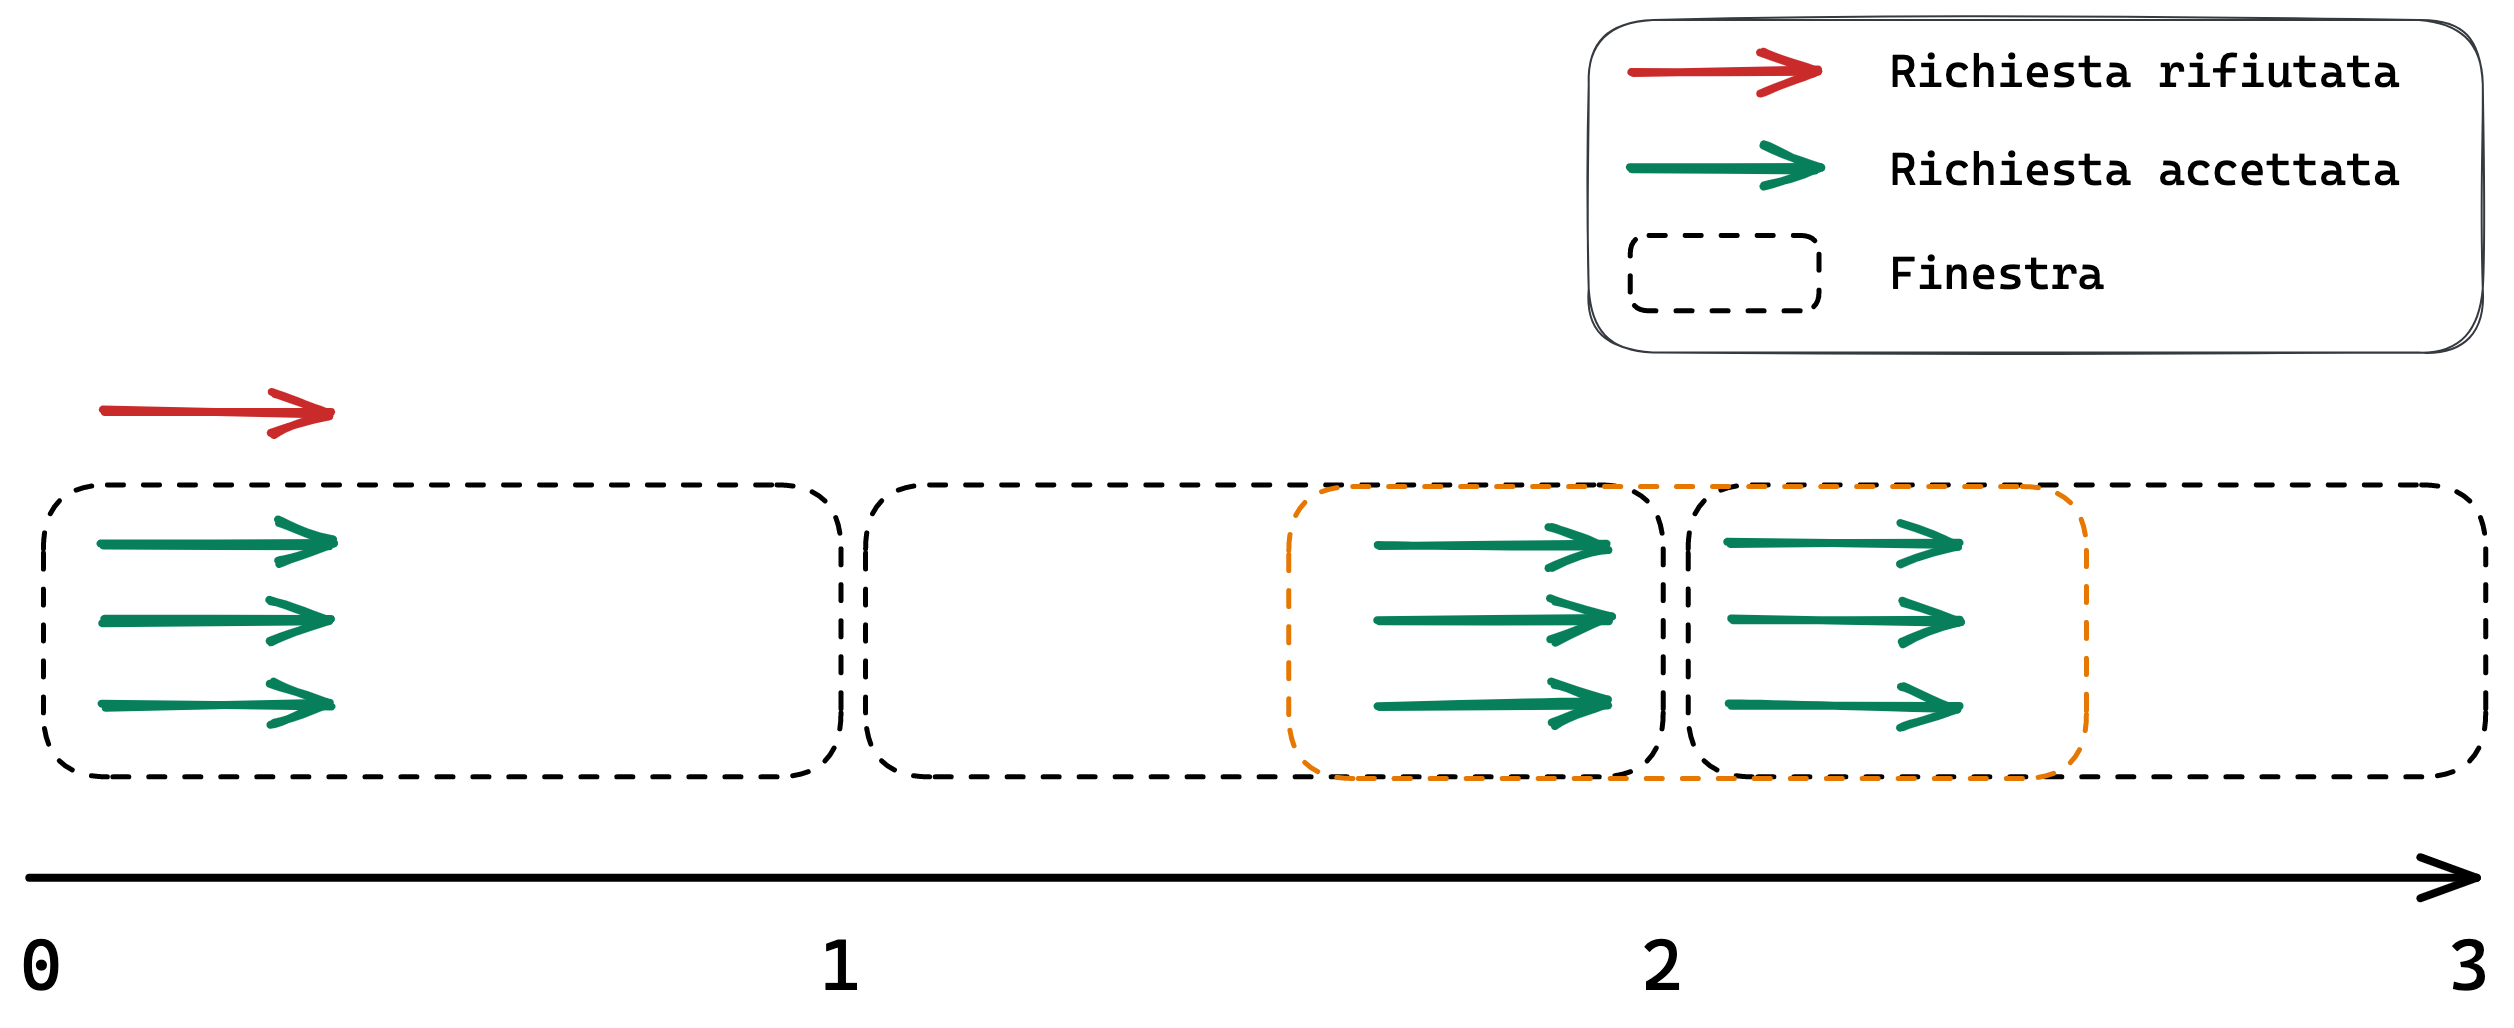
\includegraphics[width=12cm]{./immagini/fixed_window.png}
        \label{fixed window diagram}
        \caption{diagramma Rate-limiting fixed window }
        \end{figure}
    
    \item \textbf{Token bucket :} Il funzionamento del token bucket prevede che non tutte le richieste di un servizio
    vengano mappate 1:1 con la richiesta di risorse, poiché alcune richieste potrebbero richiedere più risorse di altre.
    Per questo motivo, viene mantenuto un contatore di risorse, che viene scalato per ogni richiesta, del numero di
    token necessari per portare a termine il lavoro. Il contatore ha una frequenza di riempimento, ovvero a ogni unità
    di tempo viene reimpostato al suo valore massimo. Quando un utente o un'applicazione invia una richiesta al sistema,
    il sistema verifica se ci sono abbastanza token disponibili per soddisfare la richiesta. Se non ci sono abbastanza
    token, la richiesta viene respinta. In questo modo, le richieste vengono accettate solo se c'è abbastanza capacità
    per soddisfarle.
        \begin{figure}[H]
        \centering
        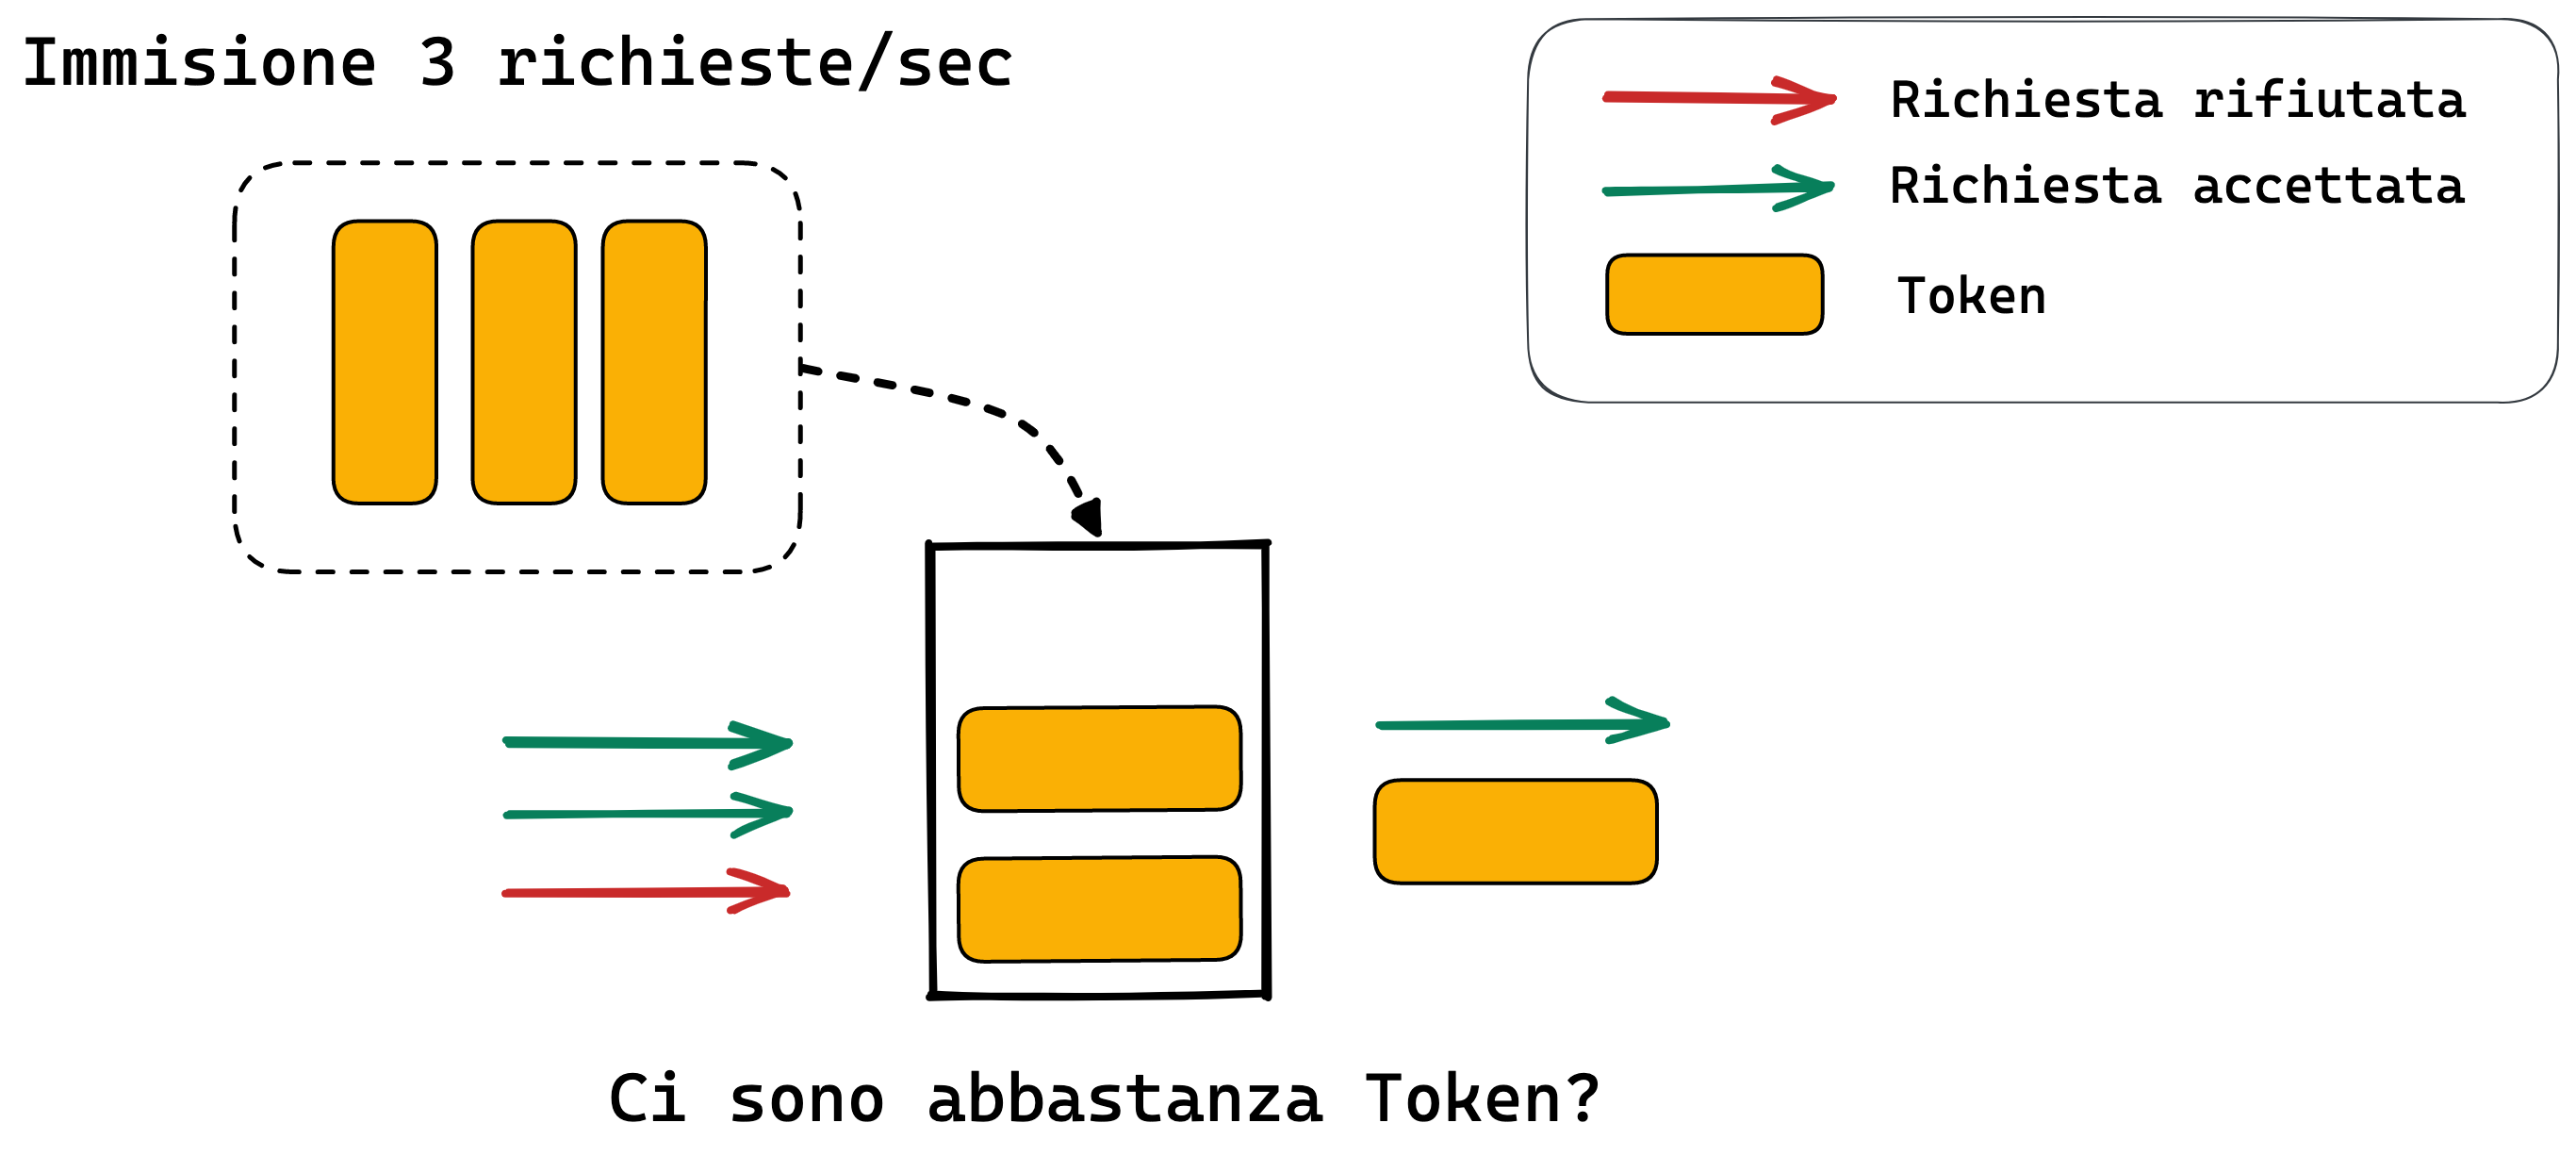
\includegraphics[width=12cm]{./immagini/token_bucket.png}
        \label{token bucket diagram}
        \caption{diagramma Rate-limiting token bucket }
        \end{figure}
    
    \item \textbf{Leaky bucket :} L'idea di base è simile a quella del Token bucket ma invece di rispondere al numero di
    richieste liberando i token necessari fino a esaurimento, il tasso di elaborazione delle richieste viene regolato in
    modo uniforme. Questo significa che quando un pacchetto di dati arriva al sistema, se il secchio è già pieno, il
    pacchetto viene scartato. Nel mentre ad ogni unità di tempo viene elaborata una quantità di richieste corrispondente
    alla velocità di uscita del sistema. In questo modo, il flusso di dati in uscita non supera mai una certa soglia.
        \begin{figure}[H]
        \centering
        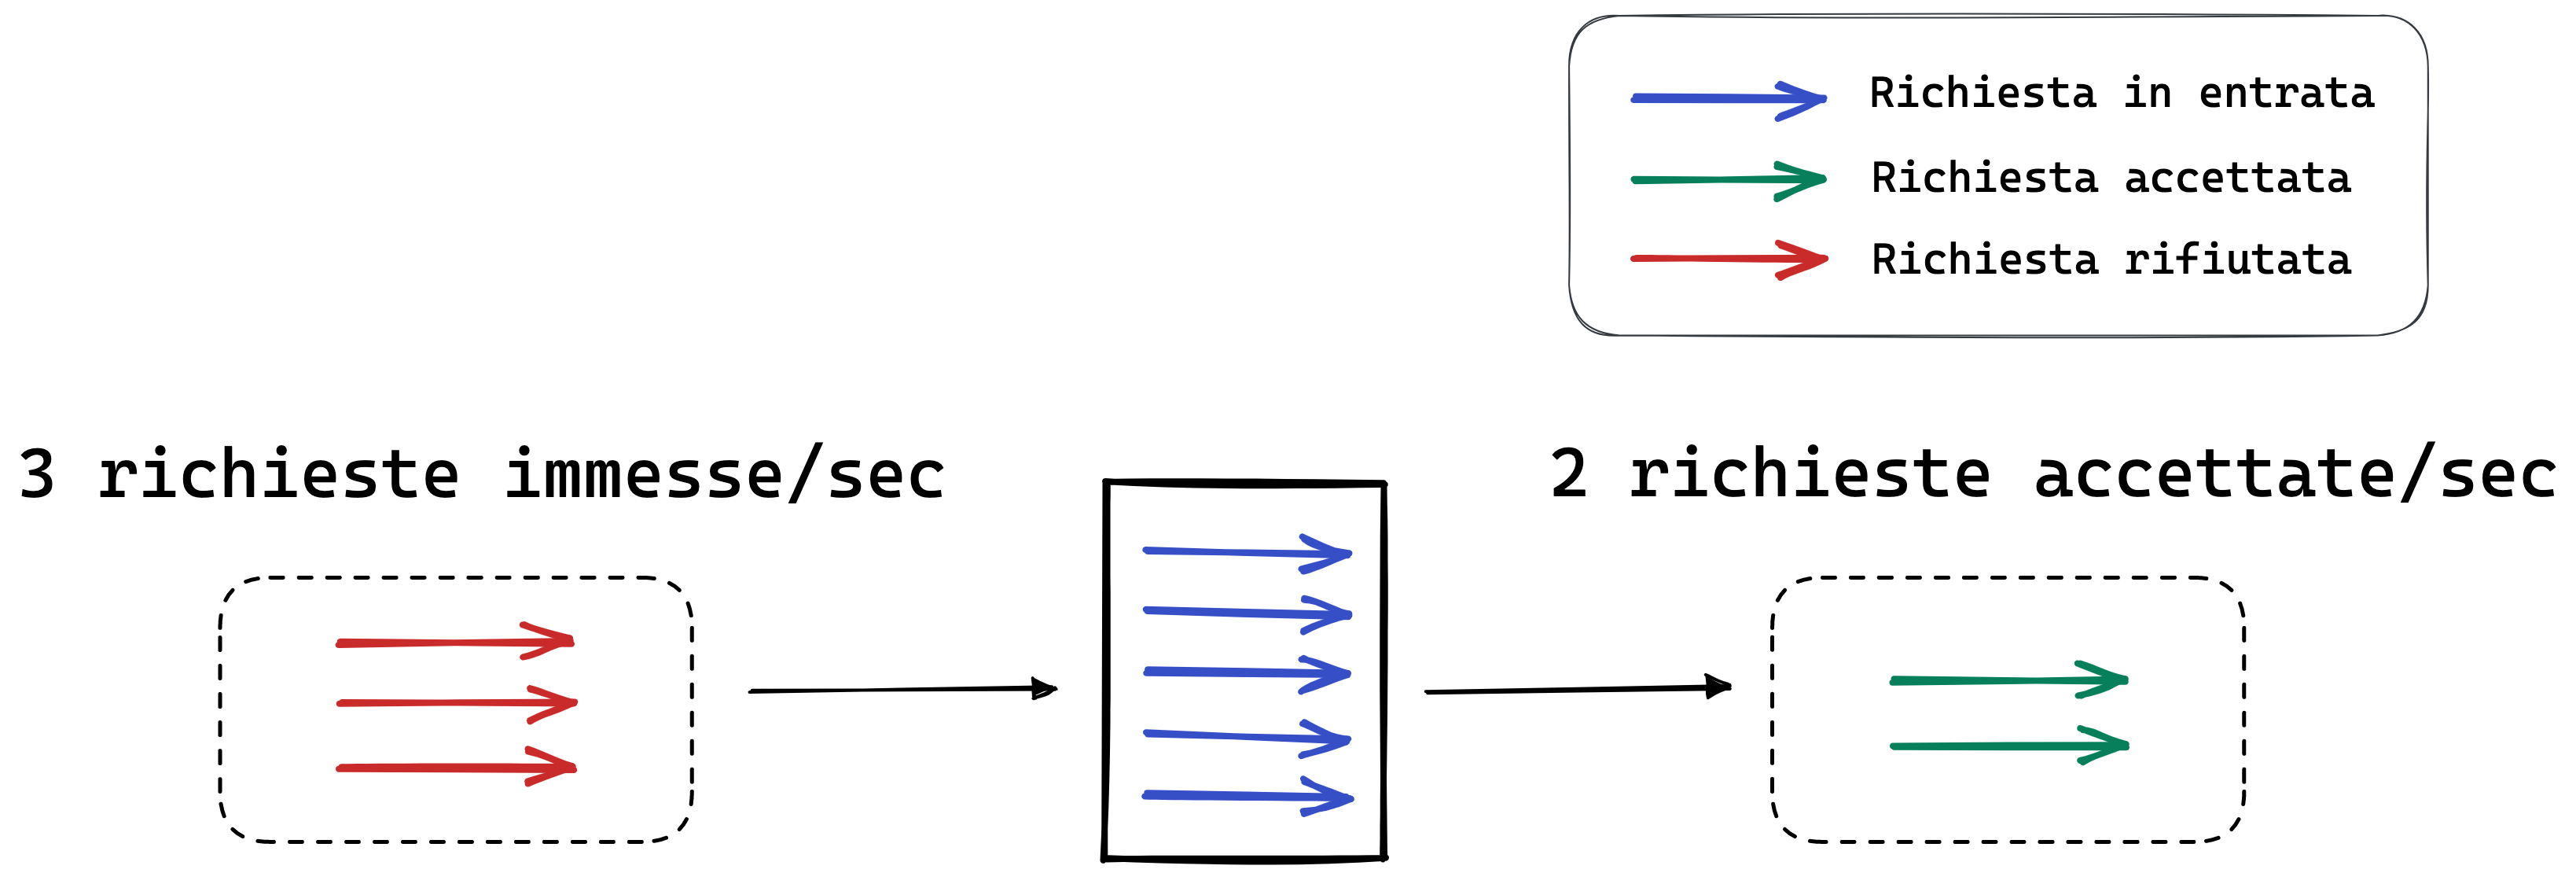
\includegraphics[width=12cm]{./immagini/leaky_bucket.png}
        \label{leaky bucket diagram}
        \caption{diagramma Rate-limiting leaky bucket }
        \end{figure}
    
    \item \textbf{Sliding window:} La strategia di sliding window adotta un approccio simile alla Fixed Window, ma con
    una differenza fondamentale: esamina il tasso di richieste effettuate in un periodo di tempo continuo piuttosto che
    in intervalli fissi. Ad esempio, se il limite di richieste è fissato a 100 al minuto, la strategia prevede di
    controllare il numero di richieste effettuate nell'ultimo minuto e, nel caso superi il limite, rifiutare la
    richiesta. Questo approccio evita il potenziale sovraccarico del sistema alla fine di una finestra con un tempo
    prefissato, ma richiede la gestione di una finestra scorrevole, aumentando la complessità di
    implementazione.\begin{figure}[H]
        \centering
        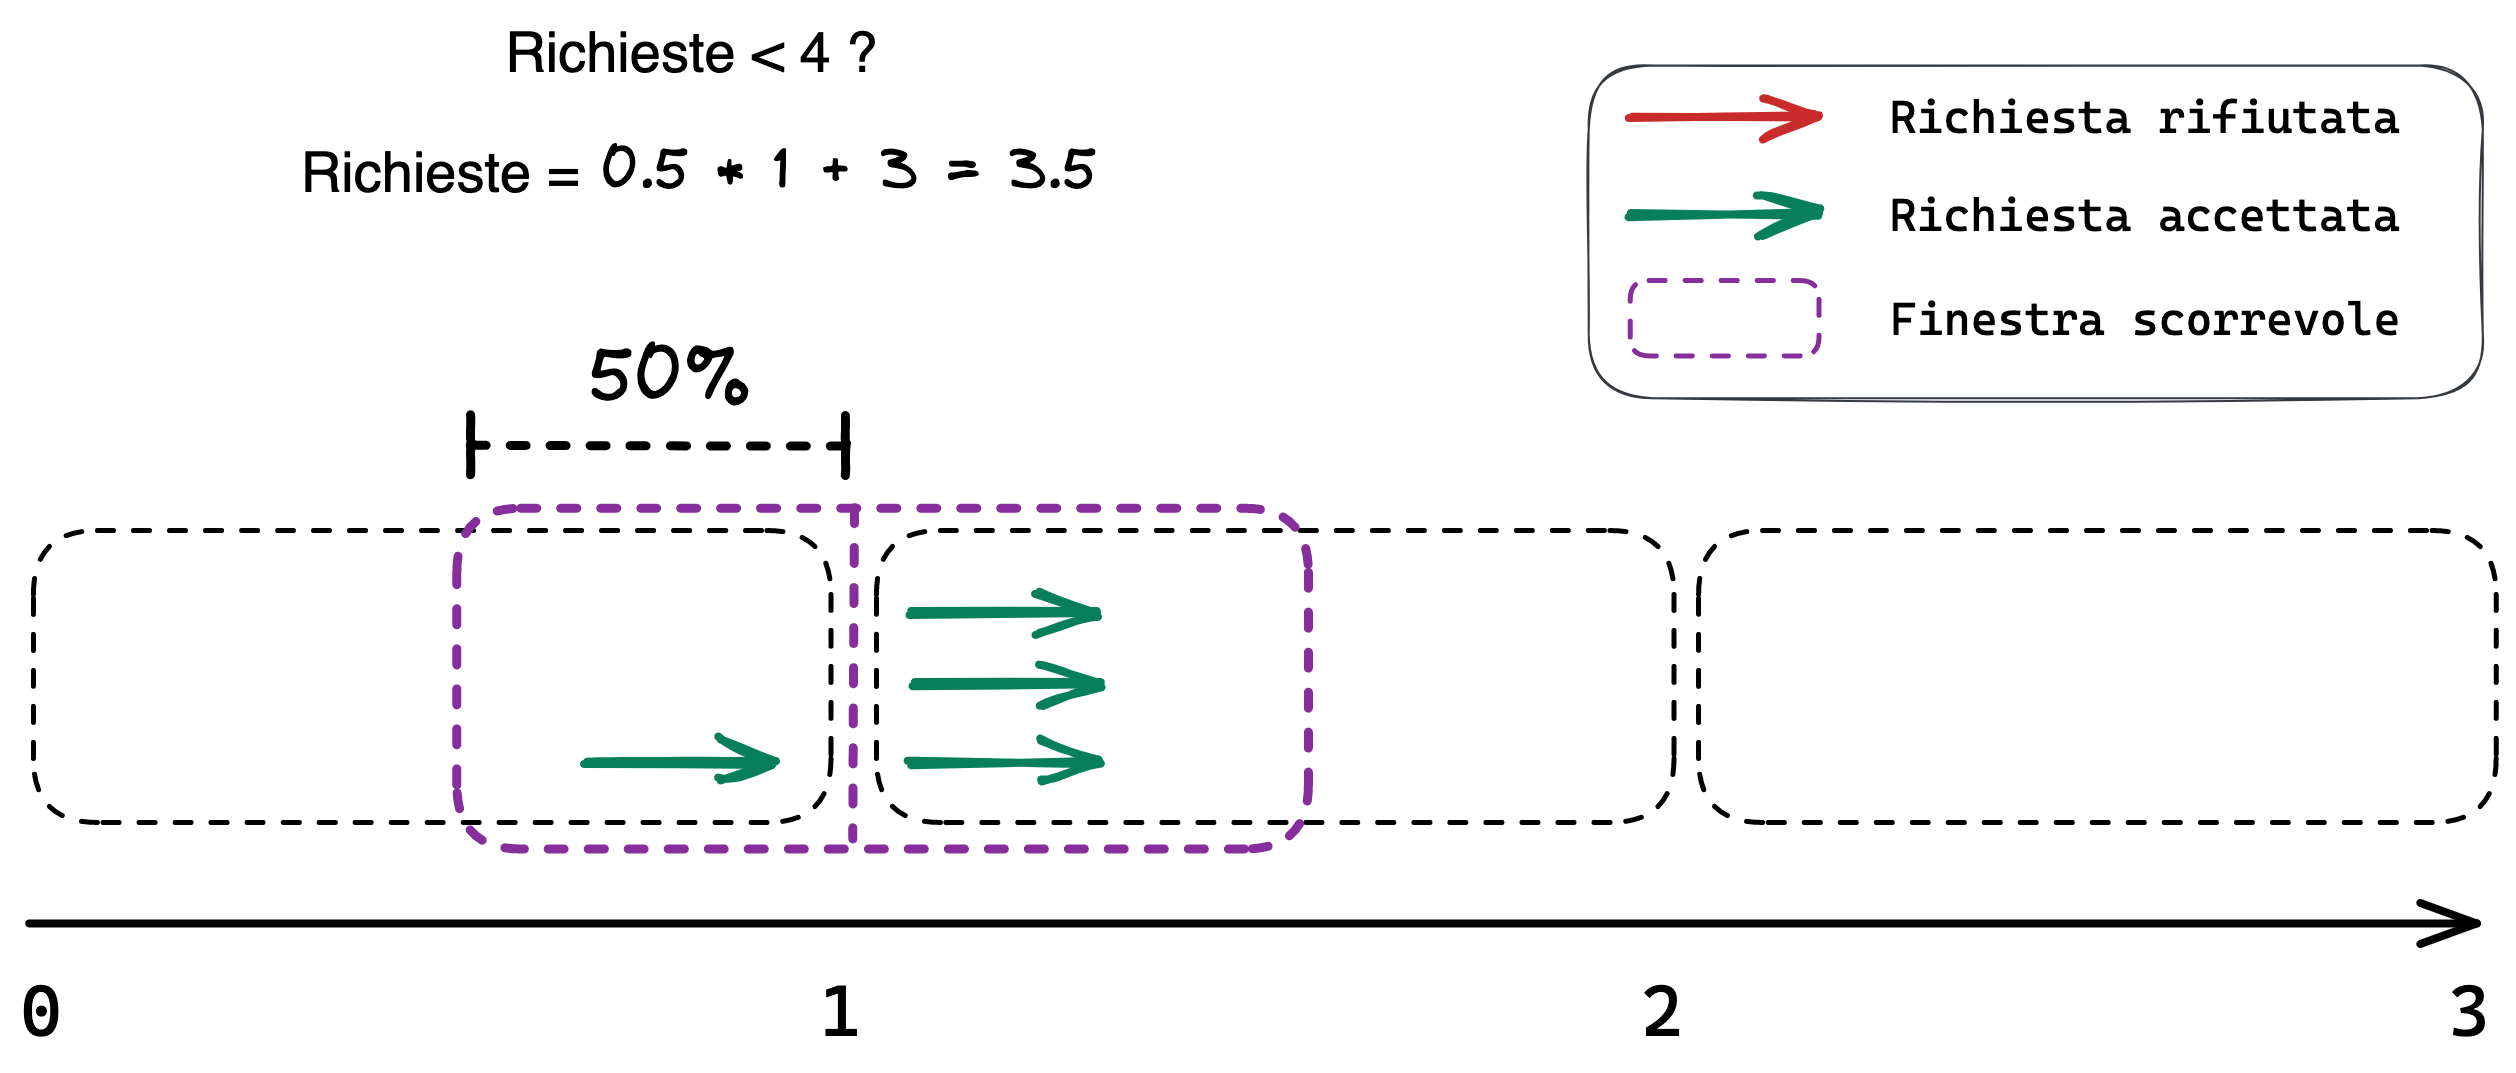
\includegraphics[width=12cm]{./immagini/sliding_window.png}
        \label{sliding window diagram}
        \caption{diagramma Rate-limiting sliding window }
        \end{figure}
\end{itemize}
\clearpage

\section{zk-SNARK}
\label{sec:zk-SNARK}
% Bibliografia
\chapter*{Bibliografia}
\chaptermark{Bibliografia}
\addcontentsline{toc}{chapter}{Bibliografia}
\phantomsection
\printbibliography[heading=bibintoc]

\end{document}
